\newpage
\section{Problem formulation and Task description}
\label{sec:pf}
In this chapter, a list of problems or areas of improvements for (\citet{DiazP2016}) is identified and a model approach based on the literature survey of the previous section is presented. A detailed take on the problems and their respective implementations will be explained in the subsequent chapters.
\subsection{Problem formulation}
The following problems related to generating successful welding paths were identified:
\begin{itemize}
\item \textbf{Reachability:} A scenario is highlighting this is presented with the aid of the following diagram (\ref{fig:pf1}). In this scenario, we can see that the selected edge cannot be reached by the 6Dof manipulator. In order to generate a successful plan, which complies with the optimal definition, it is also necessary for the entire solution to lie in the dexterous work space of the 6 Dof manipulator.
\item \textbf{Deviation from optimal angle while avoiding collision:} In the following diagram(cite), we can observe that the weld tool tip follows an angle which is not in compliance with the optimal definition in order to avoid the collision. This leads to poor quality weld.
\item \textbf{Random Sampling:} The RRT* planner is a fast and efficient algorithm and guarantees  a solution asymptotically(cite and rephrase). However as we can see from the diagram below(cite), it generates a lot of random samples which do not at all contribute to finding a proper solution. Hence to make it more efficient, the problem of random sampling can be addressed.
\end{itemize}
\begin{figure}[!ht] %  figure placement: here, top, bottom, or page
	\centering
	\frame{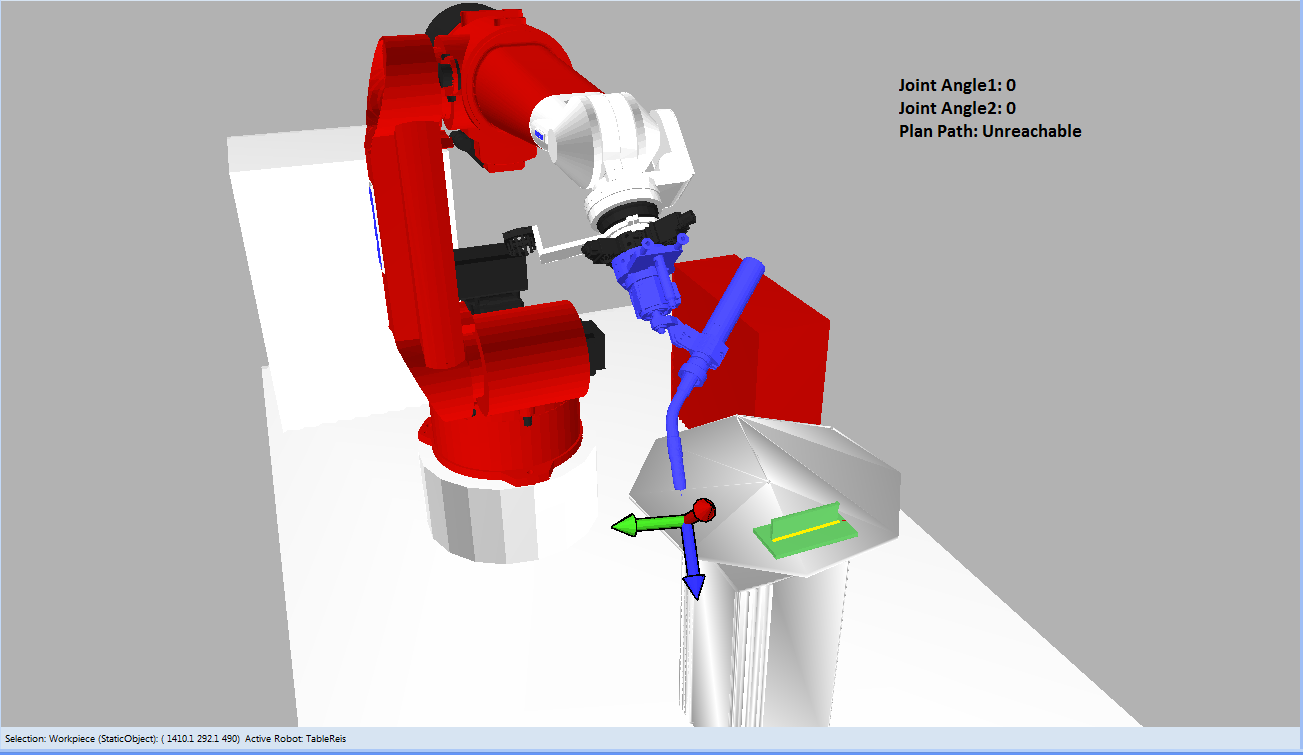
\includegraphics[width=0.8\textwidth,scale=0.6]{images/Urchbl_uscs.png}}
	\caption{Unreachable Use Case}
	\label{fig:pf1}
\end{figure} 

\subsection{Problem Approach Description}
In this section the proposed approach for the problems described above (\ref{sec:pf} is presented:

\begin{itemize}
\item \textbf{Incorporating a Rotary Table:} A rotary table can be considered as a 2 Dof which can provide extra degrees of freedom to tackle the problems of reachability and singularity. 
\item \textbf{Extending State Validity Checker:} In order to address the problems of reachability and singularity, we have to incorporate functions to detect reachability and link them to the state validity checker of the motion planner.
\item \textbf{Modeling of the Planning Space:} The introduction of the rotary table will create a more complex planning space. Generating a model for the same will help the user to visualize it as well as help to identify the gradient surface, which can be exploited to force the sampler to generate new samples in the areas with lower cost gradient thus ensuring an optimal solution.
\end{itemize}